\documentclass[presentation]{beamer}
\usetheme{Antibes}
\usecolortheme{dolphin}
%\usepackage{amsmath}
\usepackage{amsthm}
\usepackage{amssymb}
\usepackage{graphicx}
\usepackage{fullpage}
\usepackage{enumerate}
\usepackage{array}
\usepackage{multicol}
%\usepackage{youngtab}
\usepackage{float}

\usepackage[utf8x]{inputenc}
\usepackage{default}
\usepackage{amssymb,amsfonts,amsbsy,amsmath}
%\usepackage{tkz-graph}
\usepackage{amsmath}
\usepackage{graphicx}

\newcommand{\mycirc}[1]
{\textcircled{\raisebox{-.8pt}{#1}}}

\newcommand{\mytwo}[2]
{\raisebox{1.1pt}{\scriptsize #1} \hspace{1pt} \raisebox{-1.1pt}{\scriptsize #2}}


%% Some useful operatorname declarations for nice texing.
\newcommand{\Aut}{\operatorname{Aut}}
\newcommand{\Inn}{\operatorname{Inn}}
\newcommand{\Ker}{\operatorname{Ker}}
\newcommand{\Stab}{\operatorname{Stab}}
\newcommand{\orb}[1]{\mathcal{O}_#1}
\newcommand{\lcm}{\operatorname{lcm}}
\newcommand{\U}{\operatorname U}
\newcommand{\cl}{\operatorname {cl}}

%% Stuff from King's .tex files
\newcommand{\untab}{\noindent \!\!\!\!\!\!\!\!\!}
\newcommand{\lra}{\longrightarrow}
\newcommand{\mb}[1]{\mathbf{#1}}
\newcommand{\gap}{\vspace{0.1in}}
\DeclareMathOperator{\grad}{grad}
\DeclareMathOperator{\curl}{curl}
\DeclareMathOperator{\GL}{GL}
\newcommand{\myline}
{\vspace{.2in}
  \begin{center}
    \rule{5in}{.7pt}
  \end{center}
  \vspace{.2in}}

\usepackage{parskip}

\setlength{\parindent}{2ex}
\setlength{\parskip}{2ex plus 1ex minus 1ex}

%%% Good old "not sure if equal"
\newcommand{\qe}{\stackrel{?}{=}}

%% Some quickies for the big groups
\newcommand{\Q}{\mathbb Q}
\newcommand{\F}{\mathbb F}
\newcommand{\Qp}{\mathbb Q^+}
\newcommand{\Qn}{\mathbb Q^-}
\newcommand{\Qs}{\mathbb Q^*}
\newcommand{\R}{\mathbb R}
\newcommand{\Rp}{\mathbb R^+}
\newcommand{\Rn}{\mathbb R^-}
\newcommand{\Rs}{\mathbb R^*}
\newcommand{\Z}{\mathbb Z}
%\newcommand{\N}{\mathbb N}
%\newcommand{\C}{\mathbb C}

\newcommand{\Af}{\mathbb A}
\newcommand{\PP}{\mathbb P}

\newcommand{\GF}{\mathbb GF}

\newcommand{\gl}{\mathfrak g}
\newcommand{\bl}{\mathfrak b}
\newcommand{\tl}{\mathfrak t}
\newcommand{\pl}{\mathfrak p}
\newcommand{\nl}{\mathfrak n}

\DeclareMathOperator{\sh}{sh}

\newcommand{\Orb}{\mathcal O}
\newcommand{\Var}{\mathcal V}

\newcommand{\Irr}{\operatorname{Irr}}

\newcommand{\Brak}{[\cdot,\cdot]}

\newcommand{\NWN}{\nl \cap {^w\nl}}
\newcommand{\closeGNWN}{\overline{G \cdot (\NWN)}}

\newcommand{\N}{\mathbb N}
\newcommand{\C}{\mathbb C}

\newcommand{\GLn}{GL_n(\C)}
\newcommand{\gln}{\mathfrak {gl}_n}

\newcommand{\rank}{\operatorname{Rank}}

\newcommand{\bracket}{[\cdot, \cdot]}

\newcommand{\LRGfxSymArrowTwo}[2]{%
  \raisebox{1.3cm}{ \centering \parbox{.6cm}{ \centering%
    {\scriptsize $#1$}\\[-.23cm]$\longrightarrow$\\[-.3cm]%
    $\longleftarrow$\\[-.23cm] {\scriptsize $#2$}%
  } }%
}

% \newcommand{\LRGfxSymArrowTwo}[2]{
%   \raisebox{1.3cm}{
%     \begin{tabular}{c}
%       \centering%
%       {\scriptsize $#1$}\\[-.23cm]
%       $\longrightarrow$\\[-.3cm]%
%       $\longleftarrow$\\[-.23cm]
%       {\scriptsize $#2$}%
%     \end{tabular}
%   }
% }

\newcommand{\LRGfxSymArrow}[1]{
  \LRGfxSymArrowTwo{#1}{#1}
}
%% Good old "not sure if equal"
\newcommand{\qe}{\stackrel{?}{=}}

\makeatletter
\DeclareRobustCommand{\em}{%
  \@nomath\em \if b\expandafter\@car\f@series\@nil
  \normalfont \else \bfseries \fi}
\makeatother
\renewcommand<>{\emph}[1]{{\em #1}}

%% Some quickies for the big groups
\newcommand{\Q}{\mathbb Q}
\newcommand{\F}{\mathbb F}
\newcommand{\Qp}{\mathbb Q^+}
\newcommand{\Qn}{\mathbb Q^-}
\newcommand{\Qs}{\mathbb Q^*}
\newcommand{\R}{\mathbb R}
\newcommand{\Rp}{\mathbb R^+}
\newcommand{\Rn}{\mathbb R^-}
\newcommand{\Rs}{\mathbb R^*}
\newcommand{\Z}{\mathbb Z}
%\newcommand{\N}{\mathbb N}
%\newcommand{\C}{\mathbb C}

\newcommand{\Af}{\mathbb A}
\newcommand{\PP}{\mathbb P}

\newcommand{\GF}{\mathbb GF}

\newcommand{\gl}{\mathfrak g}
\newcommand{\bl}{\mathfrak b}
\newcommand{\tl}{\mathfrak t}
\newcommand{\pl}{\mathfrak p}
\newcommand{\nl}{\mathfrak n}

\DeclareMathOperator{\sh}{sh}

\newcommand{\Orb}{\mathcal O}
\newcommand{\Var}{\mathcal V}

\newcommand{\Irr}{\operatorname{Irr}}

\newcommand{\Brak}{[\cdot,\cdot]}

\newcommand{\NWN}{\nl \cap {^w\nl}}
\newcommand{\closeGNWN}{\overline{G \cdot (\NWN)}}

\newcommand{\N}{\mathbb N}
\newcommand{\C}{\mathbb C}

\newcommand{\GLn}{GL_n(\C)}
\newcommand{\gln}{\mathfrak {gl}_n}

\newcommand{\rank}{\operatorname{Rank}}


\newcommand{\loopinsert}{E_1}
\newcommand{\edgedouble}{E_2}
\newcommand{\cutedgedouble}{E_3}
\newcommand{\pairinsert}{E_4}
\newcommand{\plantri}{\textit{plantri} }
\newcommand{\nauty}{\textit{nauty} }
\newcommand{\saucy}{\textit{saucy} }
\newcommand{\valgrind}{\textit{valgrind} }


\usepackage{overpic}
%\usepackage{svg}
\usepackage{graphicx}
%\usepackage{mathrsfs}
%\usepackage{setspace}
%\usepackage{showkeys}
\usepackage{amsmath}
\usepackage{hyperref}
\usepackage{tikz}
\usepackage{pgfplots}
\usepackage{pgfplotstable}
\usepackage{array}
\pgfplotsset{compat=1.8}
\usetikzlibrary{positioning,arrows,knots,calc,decorations.markings}
\usepgfplotslibrary{colorbrewer}

\definecolor{beamerblue}{RGB}{234,233,243}
\definecolor{beamerviolet}{RGB}{47,23,132}
\definecolor{beamerliteviolet}{RGB}{137,127,207}

\tikzset{onslide/.code args={<#1>#2}{%
  \only<#1>{\pgfkeysalso{#2}} % \pgfkeysalso doesn't change the path
}}
\tikzset{temporal/.code args={<#1>#2#3#4}{%
  \temporal<#1>{\pgfkeysalso{#2}}{\pgfkeysalso{#3}}{\pgfkeysalso{#4}} % \pgfkeysalso doesn't change the path
}}

\tikzset{
  invisible/.style={opacity=0},
  visible on/.style={alt={#1{}{invisible}}},
  alt/.code args={<#1>#2#3}{%
    \alt<#1>{\pgfkeysalso{#2}}{\pgfkeysalso{#3}} % \pgfkeysalso doesn't change the path
  },
}

\pgfplotsset{
  /pgfplots/bar cycle list/.style={/pgfplots/cycle list={%
      {RdBu-9-1!50!black,fill=RdBu-9-1!80!white,mark=none},%
      {RdBu-9-2!50!black,fill=RdBu-9-2!80!white,mark=none},%
      {RdBu-9-3!50!black,fill=RdBu-9-3!80!white,mark=none},%
      {RdBu-9-4!50!black,fill=RdBu-9-4!80!white,mark=none},%
      {RdBu-9-5!50!black,fill=RdBu-9-5!80!white,mark=none},%
      {RdBu-9-6!50!black,fill=RdBu-9-6!80!white,mark=none},%
      {RdBu-9-7!50!black,fill=RdBu-9-7!80!white,mark=none},%
      {RdBu-9-8!50!black,fill=RdBu-9-8!80!white,mark=none},%
      {RdBu-9-9!50!black,fill=RdBu-9-9!80!white,mark=none},%
      {RdBu-9-80!50!black,fill=RdBu-9-80!80!white,mark=none},%
    }
  },
}

% \pgfplotsset{
%   /pgfplots/bar cycle list/.style={/pgfplots/cycle list={%
%       {red!80!black,fill=red!30!white,mark=none},%
%       {orange!80!black,fill=orange!30!white,mark=none},%
%       {yellow!80!black,fill=yellow!30!white,mark=none},%
%       {lime!80!black,fill=lime!30!white,mark=none},%
%       {green!80!black,fill=green!30!white,mark=none},%
%       {teal!80!black,fill=teal!30!white,mark=none},%
%       {cyan!80!black,fill=cyan!30!white,mark=none},%
%       {blue!80!black,fill=blue!30!white,mark=none},%
%       {violet!80!black,fill=violet!30!white,mark=none},%
%       {purple!80!black,fill=purple!30!white,mark=none},%
%     }
%   },
% }


\newcommand{\Uhyp}{\mathcal U} \newcommand{\Vhyp}{\mathcal V}
\newcommand{\Rhyp}{\mathcal R}


\title{Random Planar Diagrams}
\author[Cantarella, Chapman, Mastin]{Harrison Chapman (UGA - Graduate
  student)\\joint w/ Jason Cantarella (UGA), Matt Mastin (Wake Forest)}
\date{AMS Western Spring Sectionals 2015 (UNLV) -- April 18, 2015}

%\allowdisplaybreaks
%\usepackage[bookmarks,bookmarksopen,bookmarksdepth=4]{hyperref}

\newcommand{\so}[1]{\mathfrak {so}(#1)}

%\newtheorem{theorem}{Theorem}[section]
%\newtheorem{lemma}[theorem]{Lemma}
%\newtheorem{definition}[theorem]{Definition}
\newtheorem{proposition}[theorem]{Proposition}
%\newtheorem{corollary}[theorem]{Corollary}

%\renewcommand*\showkeyslabelformat[1]{\normalfont\tiny\ttfamily(#1)}

\graphicspath{{../../figs/}{figs/}}

\let\oldemptyset\emptyset
\let\emptyset\varnothing

\DeclareMathOperator{\Arm}{Arm}
\DeclareMathOperator{\Pol}{Pol}
\DeclareMathOperator{\UP}{UP}
\DeclareMathOperator{\VP}{VP}
\DeclareMathOperator{\APol}{APol}
\DeclareMathOperator{\Diff}{Diff}
\DeclareMathOperator{\Sympl}{Sympl}
\DeclareMathOperator{\ev}{ev}
\DeclareMathOperator{\Ad}{Ad}
\DeclareMathOperator{\crit}{crit}
\DeclareMathOperator{\ind}{ind}
\DeclareMathOperator{\intr}{int}
\DeclareMathOperator{\Hom}{Hom}
\DeclareMathOperator{\Ext}{Ext}
\DeclareMathOperator{\codim}{codim}
\DeclareMathOperator{\Ann}{Ann}
\DeclareMathOperator{\im}{Im}
\DeclareMathOperator{\Int}{int}

\begin{document}

\newcommand{\Oh}[1]{\mathcal O (#1)}
\newcommand{\g}{\mathfrak g}
\newcommand{\ShSet}{\mathcal S}
\newcommand{\LnSet}{\mathcal L}
\newcommand{\sr}{/\!\!/}

\begin{frame}
\titlepage
\small{Sponsored by NSF VIGRE [typeset this]}
\end{frame}

\section{Introduction}

\begin{frame}
  \frametitle{Natural questions about knot diagrams}
  \begin{block}{Question}
    What fraction of 8-crossing diagrams are trefoils?
    \onslide<2>{\begin{center}$12.48\%$
      \end{center}
    }
  \end{block}
  \begin{figure}
    \centering
    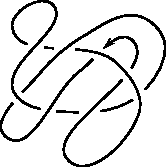
\includegraphics[width=1.5in]{8x_tref.pdf}
  \end{figure}
\end{frame}

\begin{frame}
  \frametitle{Natural questions about knot diagrams}
  \begin{block}{Question}
    What is the average minimal crossing \# of an 8-crossing diagram?
    \onslide<2>{\begin{center}$12.48\%$
      \end{center}
    }
  \end{block}
  \begin{figure}
    \centering
    \[
    \vcenter{\hbox{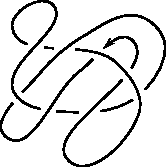
\includegraphics[width=1.5in]{8x_tref.pdf}}}
    \Rightarrow
    \vcenter{\hbox{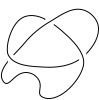
\includegraphics[width=1.5in]{8x_min_tref.pdf}}}
    \]
  \end{figure}
\end{frame}

\begin{frame}
  \frametitle{Natural questions about knot diagrams}
  Define an operation on diagrams, \emph{delooping}: Recursively RI
  untwist monogon loops in a diagram until there are no more.
  \begin{figure}
    \centering
    \[
    \vcenter{\hbox{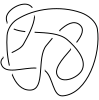
\includegraphics[width=1.5in]{8x_tref_loopy.pdf}}}
    \Rightarrow
    \vcenter{\hbox{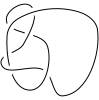
\includegraphics[width=1.5in]{8x_tref_deloopy.pdf}}}
    \]
  \end{figure}

\end{frame}

\begin{frame}
  \frametitle{Natural questions about knot diagrams}
  \begin{block}{Question}
    What is the average crossing \# of a delooped 8-crossing diagram?
    \onslide<2>{\begin{center}$12.48\%$
      \end{center}
    }
  \end{block}
  \begin{figure}
    \centering
    \[
    \vcenter{\hbox{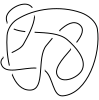
\includegraphics[width=1.5in]{8x_tref_loopy.pdf}}}
    \Rightarrow
    \vcenter{\hbox{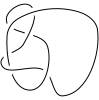
\includegraphics[width=1.5in]{8x_tref_deloopy.pdf}}}
    \]
  \end{figure}
\end{frame}

\begin{frame}
  \frametitle{Natural questions about knot diagrams}
  \begin{block}{Question}
    How many 8-crossing diagrams can be delooped to the unknot?
    \onslide<2>{\begin{center}$44.51\%$
      \end{center}
    }
  \end{block}
  \begin{figure}
    \centering
    \includegraphics[width=1.5in]{tree_like_8x.pdf}
  \end{figure}
\end{frame}


\begin{frame}
  \frametitle{Knotting and Polymers}
  \begin{figure}
    \centering

    \caption{Knotting in polymers. DNA must be unlinked during mitosis
      (left). Enzymes must fold appropriately (right).}
    \label{fig:polymr}
  \end{figure}
\end{frame}

\begin{frame}
  \frametitle{Random curve distributions}
  Classical workflow for understanding knotting in random polymers:
  Random distributions on spaces of curves
  \begin{itemize}
  \item Random space polygons. (Fixed edge length, equilateral,
    confined, etc.)
  \item Random closed self-avoiding lattice walks.
  \end{itemize}

  \begin{figure}
    \centering
    \begin{tikzpicture}[->,,shorten >=1pt,semithick,align=center]
      % \tikzstyle{every node}=[align=center]
      \node[text width=1in,draw=black] (plantri)
      {Polymers\\\includegraphics[width=.95in]{polymer_protein.jpg}};
      \node[text width=1in,right=.3in of plantri,draw=black]  (expand)
      {Polygons\\\includegraphics[width=.95in]{space_polygon.jpg}};
      \node[text width=1in,right=.3in of expand,draw=black] (isomch)
      {Knots\\\includegraphics[width=.95in]{knot_3d.jpg}};

      \path (plantri)    edge (expand)
      (expand)     edge (isomch);
    \end{tikzpicture}
    \caption{Typical random curve workflow}
  \end{figure}
\end{frame}

\begin{frame}
  \frametitle{Combinatorial knot distributions}
  Alternative approach: Combinatorial distributions
  \begin{itemize}
  \item Petaluma model (Evan-Zohar, Hass, et al.)
  \item Random braid words
  \end{itemize}
  Combinatorial models are recent.
\end{frame}

\begin{frame}
  \frametitle{The Petaluma model}
  Many satisfying theorems have been proven for the Petaluma model
  \begin{figure}
    \centering
    \resizebox{.8\columnwidth}{!}{\begin{tabular}{ccc}
\tikz[thick]{
\foreach \angle in {0, 72, ..., 288} \draw[decoration={markings,mark=at position 0.7 with {\arrow{>}}},postaction={decorate}] (0,0) .. controls +(\angle+36:4) and +(\angle:4) .. (0,0);
\filldraw (0,0)+(306:2.83) circle (2pt);
\foreach \angle/\num in {0/4, 72/3, 144/2, 216/1, 288/0} \draw (0,0)+(\angle-6:1) node[scale=1] {$\num$};
%\draw[step=0.5,gray,very thin] (-3,-3) grid (3,3);
\pgfresetboundingbox \clip (-3,-2.75) rectangle (3,3);} &
\tikz[thick]{
\draw[->,double,thick] (-0.5,-0.5) -- (0.5,-0.5);
%\draw[step=0.5,gray,very thin] (-0.5,-3) grid (0.5,3);
\pgfresetboundingbox \clip (-0.5,-2.75) rectangle (0.5,3);} &
\tikz[thick]{
\foreach \x in {0,1,...,4} {
%\draw[white,-,line width = 5] (\x*288-54:3) -- (\x*288+90:3);
\draw[>=triangle 90 cap,white,<->,line width = 6,shorten >=3, shorten <=3] (\x*288-54:3) -- (\x*288+90:3);
\draw[black,decoration={markings,mark=at position 0.25 with {\arrow{>}}},postaction={decorate}] (\x*288-54:3) -- node[fill=white,draw,circle,scale=0.6]{\x} (\x*288+90:3); }
\foreach \x in {0,1,...,4} {
\draw (\x*144-54:3)+(\x*144+99:1) node[auto,scale=0.7] {\x};}
\foreach \p/\x in {24/0,03/1,14/2,02/3,13/4} \node[scale=0.7] at (\x*144-90:1.5){$p_{\p}$};
\filldraw (306:3) circle (2pt);
%\draw[step=0.5,gray,very thin] (-3,-3) grid (3,3);
\pgfresetboundingbox \clip (-3,-2.75) rectangle (3,3);
} \\
Petal diagram & & Star diagram
\end{tabular}}

    \caption{Petal diagram and corresponding star diagram for the
      trefoil. (Diagram from Evan-Zohar, et al.)}
    \label{fig:petaluma}
  \end{figure}
\end{frame}

\begin{frame}
  \frametitle{The void}
  There is no clear connection between the two models: E.g.\ how to
  produce a star diagram from a random polygon?
  \begin{figure}
    \centering
    \begin{tikzpicture}[->,,shorten >=1pt,semithick,align=center]
      % \tikzstyle{every node}=[align=center]
      \node[text width=1in,draw=black] (knots) {Knot types};
      \node[below=.5in of knots] (diagrams) {};
      \node[text width=1.2in,draw=black,left=.5in of diagrams] (curves) {Curve\\distributions};
      \node[text width=1.2in,draw=black,right=.5in of diagrams]  (combs)
      {Combinatorial distributions};

      \path (curves) edge (knots)
             (combs) edge (knots);
      \draw[-,decorate, decoration={zigzag}] (curves) -- (combs) node[midway,above]  {???};
      %\path (plantri)    edge (expand)
      %(expand)     edge (isomch);
    \end{tikzpicture}
    \caption{There is no convenient middle between the two methods}
  \end{figure}
\end{frame}

\begin{frame}
  \frametitle{The random diagram model}
  Every space curve can
  project to a diagram, \emph{and} diagrams are combinatorial objects.
  \begin{figure}
    \centering
    \begin{tikzpicture}[->,,shorten >=1pt,semithick,align=center]
      % \tikzstyle{every node}=[align=center]
      \node[text width=1in,draw=black] (knots) {Knot types};
      \node[below=.5in of knots] (diagrams) {};
      \node[text width=1.2in,draw=black,left=.5in of diagrams] (curves) {Curve\\distributions};
      \node[text width=1.2in,draw=black,right=.5in of diagrams]
      (combs)
      {Combinatorial distributions};
      \node[text width=1.4in, draw=black,below=.3in of diagrams]
      (dias) {Random\\diagram model};

      \path (curves) edge (knots)
             (combs) edge (knots)
             (dias) edge (knots);

      \draw[<->,thick,beamerviolet] (dias.west) -- (curves);
      \draw[<->,thick,beamerviolet] (dias.east) -- (combs);
      %\path (plantri)    edge (expand)
      %(expand)     edge (isomch);
    \end{tikzpicture}
    \caption{We're trying to fill the void with the random diagram model}
  \end{figure}
\end{frame}

\begin{frame}
  \frametitle{Random diagrams}
  \begin{definition}
    In the \emph{random diagram model} of random knotting, a
    $n$-crossing diagram is drawn uniformly from the finite set of
    $n$-crossing knot diagrams.
  \end{definition}
\end{frame}

\begin{frame}
  \frametitle{Diagrams from shadows}
  Sample diagrams uniformly through tabulation:
  \begin{enumerate}
  \item Enumerate shadows (underlying graph structure behind
    diagrams).
  \item Expand shadows into diagrams.
  \end{enumerate}
\end{frame}

\begin{frame}
  \frametitle{Knot shadows and circle immersions}
  \begin{block}{}
    Knot shadows in $n$ crossings $\Leftrightarrow$ unoriented, generic
    immersions of the circle into the sphere with $n$ double points,
    up to unoriented diffeomorphism.
  \end{block}
  \begin{figure}
    \centering
    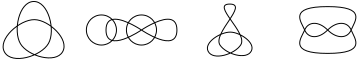
\includegraphics[width=4in]{linkshadow.pdf}
    \caption{Knot shadows. The shadow on the left is equivalent to the
      shadow on the right.}
    \label{fig:shadows}
  \end{figure}
\end{frame}

\begin{frame}
  \frametitle{How many shadows?}
    \begin{table}
    \centering
    \begin{tabular}{r|c}
      n & \# knot shadows \\
      \hline
      0 & 1 \\
      1 & 1 \\
      2 & 2 \\
      3 & 6 \\
      4 & 19\\
      5 & 76 \\
      6 & 376$^{*}$ \\
      7 & 2194$^{*}$ \\
      8 & 14614$^{**}$ \\
      9 & 106421$^{**}$ \\
    \end{tabular}
    \caption{Counts on knot shadows. Numbers
      are large, but finite.}
    \label{tab:counts}
  \end{table}
\end{frame}

% \begin{frame}
%   \frametitle{How many link shadows?}
%   \begin{block}{}
%     Counts of link shadows with $n$ crossings match K\'apolnai,
%     Domokos, and Szab\'o's counts of spherical multiquadrangulations
%     with $n+2$ crossings (hence $n$ faces).
%   \end{block}

%     \textit{Caveat:} They use \texttt{plantri} in their
%       computations too, although it is not clear how.

% \end{frame}

\begin{frame}
  \frametitle{How many knot shadows?}
  \begin{block}{}
    Counts of knot shadows with $n$ crossings match Arnol'd's counts of
    immersions of the unoriented circle into the unoriented sphere
    with $n$ double points (OEIS A008989).
  \end{block}

    \textit{Caveat:} Arnol'd's list is for $n=0$ to $n=5$; the
      terms for $n=6$ and $n=7$ are attributed to Guy H.\ Valette with
      no clear source.
\end{frame}

\begin{frame}
  \frametitle{How many shadows?}
    \begin{table}
    \centering
    \begin{tabular}{r|c}
      n & \# knot shadows \\
      \hline
      0 & 1 \\
      1 & 1 \\
      2 & 2 \\
      3 & 6 \\
      4 & 19\\
      5 & 76 \\
      6 & 376$^{*}$ \\
      7 & 2194$^{*}$ \\
      8 & 14614$^{**}$ \\
      9 & 106421$^{**}$ \\
    \end{tabular}
    \caption{$*$: Attributed to Guy H.\
      Valette. $**$: New; values not in OEIS.}
    \label{tab:counts}
  \end{table}
\end{frame}

\begin{frame}
  \frametitle{Tabulating knot shadows}
  Ggenerated table of knot shadows two different ways as a
  check.\\\hfill\\

  Both methods use features from McKay and Brinkmann's \texttt{plantri}.
\end{frame}

\begin{frame}
  \frametitle{Duals to quadrangulations}
  \begin{figure}
    \hphantom{.}
    \hfill
    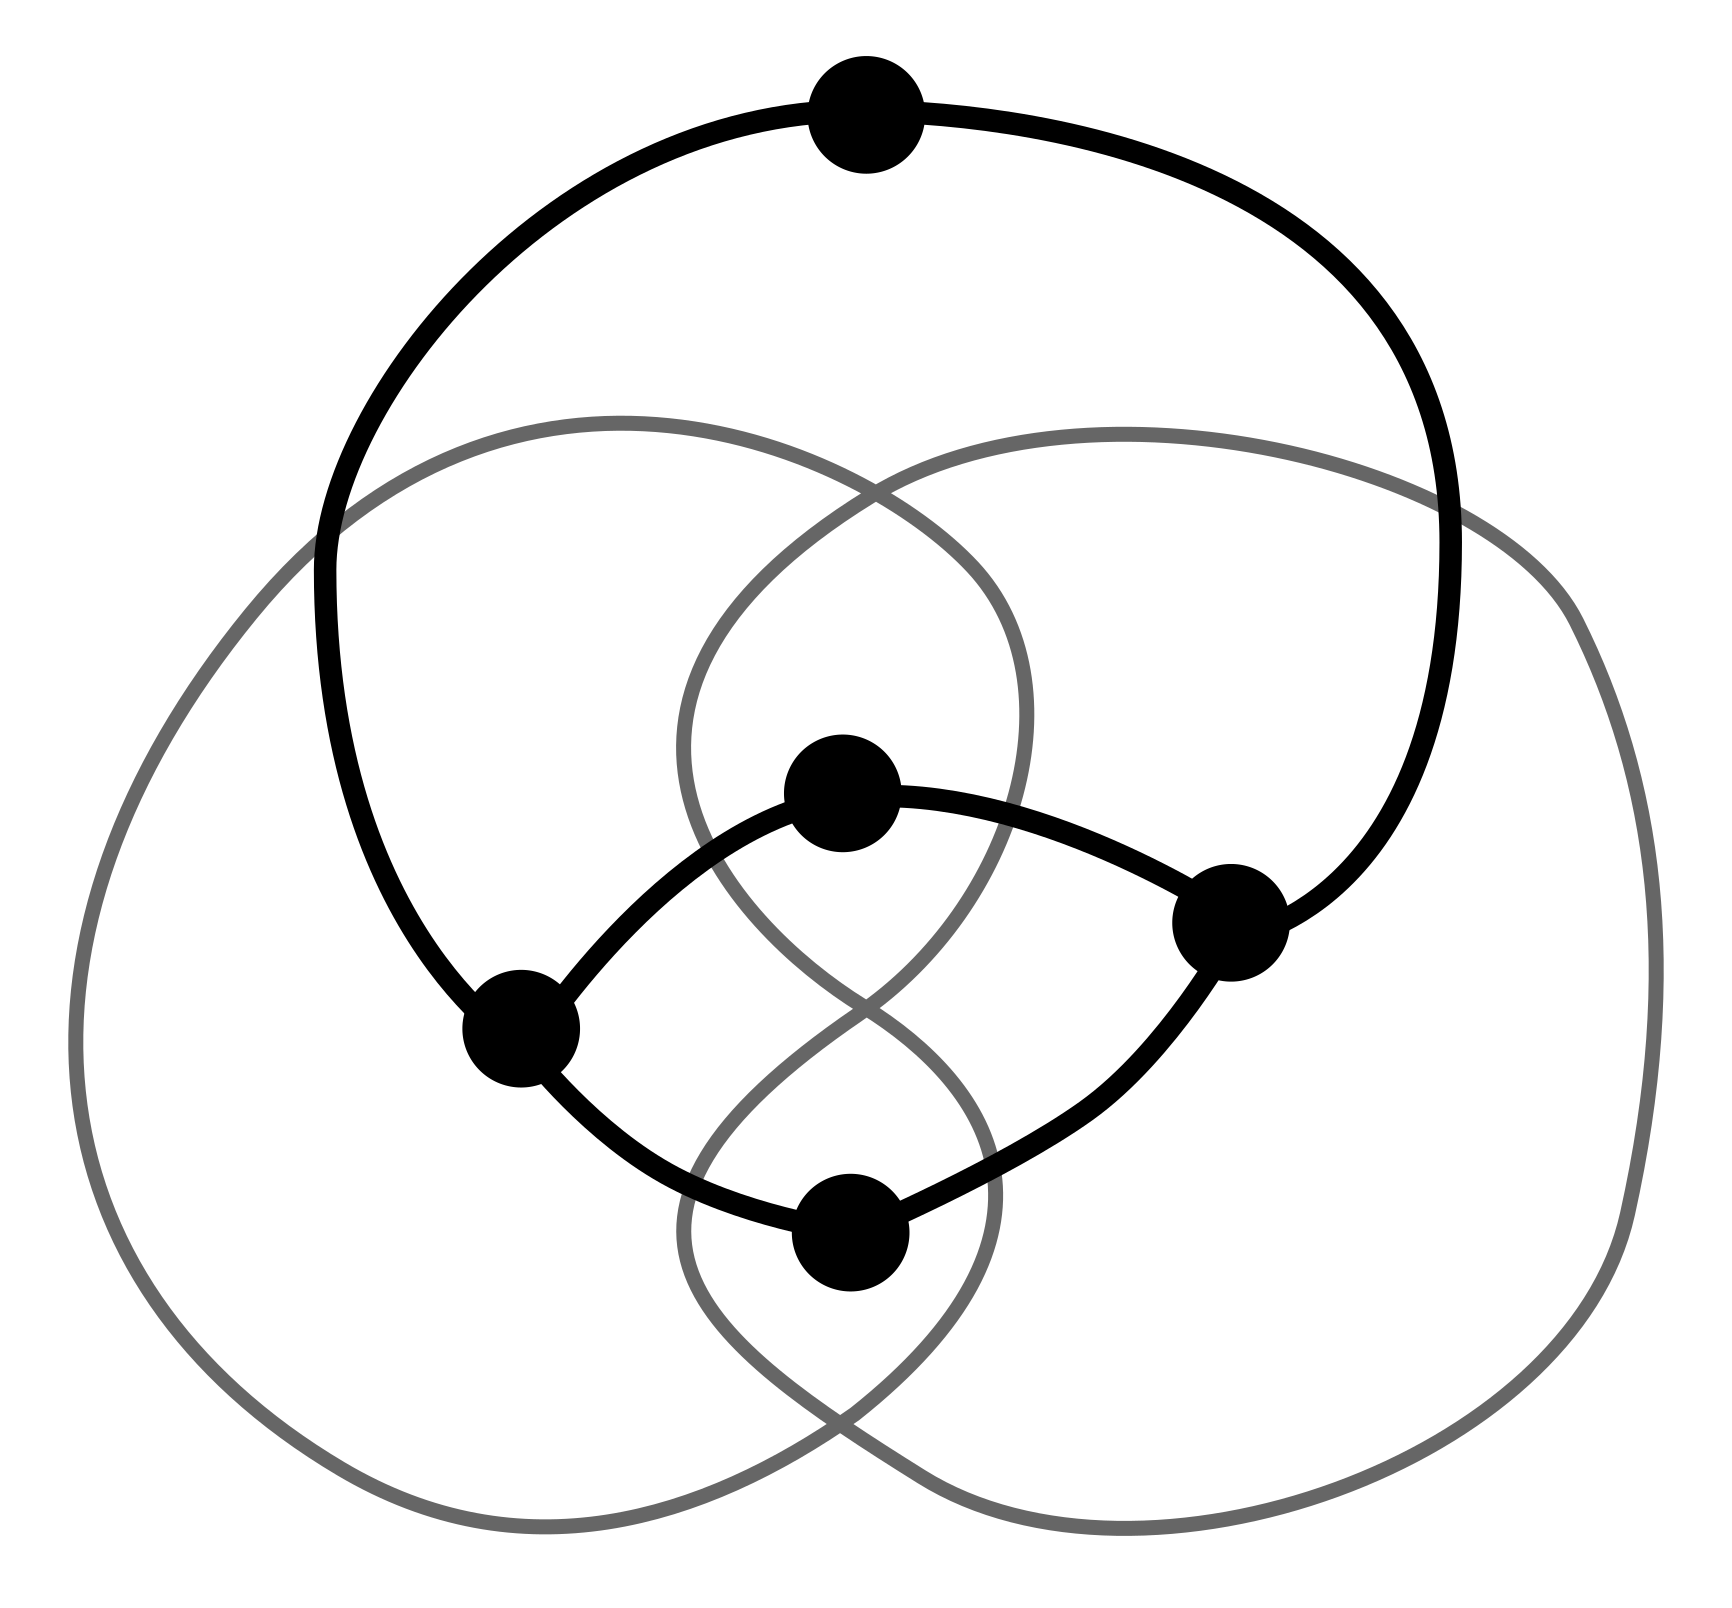
\includegraphics[height=1.25in]{quadrangulation} \hfill
    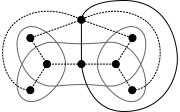
\includegraphics[height=1.25in]{non-simple-quadrangulation}
    \hfill
    \hphantom{.}
    \caption{\label{fig:NonSimpleQuad} Find all quadrangulations of
    the sphere in $n$ faces. Shadows are dual to quadrangulations.}
  \end{figure}
\end{frame}

\begin{frame}
  \frametitle{Planar graph expansions}
  \begin{figure}
    \centering
      \includegraphics[width=4in]{expansion-from-simple-graph.pdf}
    \caption{Reduction to a planar graph of degree $\le 4$ and
      connectivity $\ge 1$. Expansion is the inverse.}
    \label{fig:graphexpand}
  \end{figure}
\end{frame}

\begin{frame}
  \frametitle{The space of shadows}
  \begin{figure}
    \centering
    \includegraphics[width=\textwidth,height=\textheight,keepaspectratio]{epsgroup_0_collage.eps}
    \caption{Link shadows. Pictures generated by Eric Lybrand (UGA)
      with with SnapPy. A map of all shadows with between 3 and 6
      crossings
      \href{http://prezi.com/s5te-8obcfgq/?utm_campaign=share&utm_medium=copy&rc=ex0share}{is
        here.}}
    \label{fig:planarcollage0}
  \end{figure}
\end{frame}

\begin{frame}
  \frametitle{The space of shadows}
  \begin{figure}
    \centering
    \includegraphics[width=\textwidth,height=\textheight,keepaspectratio]{epsgroup_1_collage.eps}
    \caption{Link shadows. Pictures generated by Eric Lybrand (UGA)
      with with SnapPy.  A map of all shadows with between 3 and
      6 crossings \href{http://prezi.com/s5te-8obcfgq/?utm_campaign=share&utm_medium=copy&rc=ex0share}{is here.}}
    \label{fig:planarcollage1}
  \end{figure}
\end{frame}

\begin{frame}
  \frametitle{The space of shadows}
  \begin{figure}
    \centering
    \includegraphics[width=\textwidth,height=\textheight,keepaspectratio]{epsgroup_10_collage.eps}
    \caption{Link shadows. Pictures generated by Eric Lybrand (UGA)
      with with SnapPy. A map of all shadows with between 3 and
      6 crossings \href{http://prezi.com/s5te-8obcfgq/?utm_campaign=share&utm_medium=copy&rc=ex0share}{is here.}}
    \label{fig:planarcollage10}
  \end{figure}
\end{frame}

\begin{frame}
  \frametitle{The space of shadows}
  \begin{figure}
    \centering
    \includegraphics[width=\textwidth,height=\textheight,keepaspectratio]{epsgroup_16_collage.eps}
    \caption{Link shadows. Pictures generated by Eric Lybrand (UGA)
      with with SnapPy. A map of all shadows with between 3 and
      6 crossings \href{http://prezi.com/s5te-8obcfgq/?utm_campaign=share&utm_medium=copy&rc=ex0share}{is here.}}
    \label{fig:planarcollage16}
  \end{figure}
\end{frame}

\begin{frame}
  \frametitle{Tabulation is difficult!}
  Accounting for symmetry is complicated.

  \begin{figure}
    \centering
    \caption{The trefoil shadow has 12-fold symmetry (Left). This
      diagram with trefoil shadow has 6-fold symmetry (Right).}
    \label{fig:trefsym}
  \end{figure}
\end{frame}

\begin{frame}
  \frametitle{Breaking symmetries could make counting easier}
  Easier to count shadows/diagrams with broken symmetries
  (rooted diagrams). E.g., is a correspondence:

  \begin{figure}
    \centering

    \caption{Two-leg diagrams (left) correspond to rooted shadows (right).}
    \label{fig:legdia}
  \end{figure}

  Diagrams on the left are counted by a generating function (Bouttier,
  et.\ al).
\end{frame}

\section{Data and Analysis}

\begin{frame}
  \frametitle{From shadows to diagrams}
  Expansion of shadows to diagrams procedure:
  \begin{enumerate}
  \item Orient each component. ($2^{\#\text{components}}$ choices)
  \item Assign over-under information to each
    vertex. ($2^{\#\text{crossings}}$ choices)
  \item Group diagrams by isomorphism.
  \end{enumerate}
\end{frame}


\begin{frame}
  \frametitle{How many knot diagrams?}
  \begin{table}
    \centering
    \begin{tabular}{r|ccc}
      n  & \# knot shadows & \# knot diagrams & \# knot iso. classes \\
      \hline
      %0 & 1               & 2                & 1                    \\
      %1 & 1               & 4                & 1                    \\
      %2 & 2               & 16               &                      \\
      3  & 6               & 96               & 36                   \\
      4  & 19              & 608              & 276                  \\
      5  & 76              & 4,864            & 2,936                \\
      6  & 376             & 48,128           & 35,872               \\
      7  & 2,194           & 561,664          & 484,088              \\
      8  & 14,614          & 7,482,368        & 6,967,942            \\
      9  & 106,421         & 108,975,104      & \text{in process}    \\
    \end{tabular}
    \caption{Counts of knot shadows and diagrams}
    \label{tab:counts}
  \end{table}
\end{frame}

\begin{frame}
  \frametitle{Knotting probabilities}
  \begin{itemize}
  \item Advantage of a combinatorial model:
    Able to run searches across entire space computationally.
  \item Can check knot type of each diagram (HOMFLY is typically
    enough for our low crossing number)
  \item Possible to run many different types of searches
  \end{itemize}

\end{frame}

\begin{frame}
  \begin{figure}
    \centering
    \begin{tikzpicture}[scale=1]
      \begin{axis}[
        ymode=log,
        log ticks with fixed point,
        title={Ratio of unknots in $n$-crossing diagram iso. classes (log scale)},
        xlabel={Max \# crossings in diagram},
        ylabel={Ratio of unknots},
        cycle list name=Mark-Set1-9,
        ]
        \addplot table[x=n,y=0.1] {knot_freq.tsv};
      \end{axis}
    \end{tikzpicture}
    \label{fig:unkdecay}
  \end{figure}
\end{frame}

\begin{frame}
  \begin{figure}
    \centering
    \begin{tikzpicture}[scale=1]
      \begin{axis}[
        ymode=log,
        log ticks with fixed point,
        title={Ratios of knots in $n$-crossing diagram iso. classes (log scale)},
        xlabel={Max \# crossings in diagram},
        ylabel={Ratios of knots},
        cycle list name=Mark-Set1-9,
        legend pos=south west,
        legend entries={$3_1$, $4_1$, $5_1$, $5_2$},
        ]
        \addplot table[x=n,y=3.1] {knot_freq.tsv};
        \addplot table[x=n,y=4.1] {knot_freq.tsv};
        \addplot table[x=n,y=5.1] {knot_freq.tsv};
        \addplot table[x=n,y=5.2] {knot_freq.tsv};
      \end{axis}
    \end{tikzpicture}
    \label{fig:kgrow1}
  \end{figure}
\end{frame}


\begin{frame}
  \begin{figure}
    \centering
      \tikzset{mark=*}
    \begin{tikzpicture}[scale=1]
      \begin{axis}[
        ymode=log,
        log ticks with fixed point,
        title={Ratios of knots in $n$-crossing diagram iso. classes (log scale)},
        xlabel={Max \# crossings in diagram},
        ylabel={Ratios of knots},
        cycle list name=Mark-Set1-9,
        legend style={font=\tiny},
        legend pos=outer north east,
        legend entries={$3_1$, $4_1$, $5_1$, $5_2$, $6_1$, $6_2$, $3_1
          \# 3_1$, $3_1 \# 3_1^*$, $7_1$, $7_2$, $7_3$, $7_4$, $7_5$,
          $7_6$, $7_7$},
        ]
        \addplot table[x=n,y=3.1] {knot_freq.tsv};
        \addplot table[x=n,y=4.1] {knot_freq.tsv};
        \addplot table[x=n,y=5.1] {knot_freq.tsv};
        \addplot table[x=n,y=5.2] {knot_freq.tsv};
        \addplot table[x=n,y=6.1] {knot_freq.tsv};
        \addplot table[x=n,y=6.2] {knot_freq.tsv};
        \addplot table[x=n,y=3.1c3.1] {knot_freq.tsv};
        \addplot table[x=n,y=3.1c3.1m] {knot_freq.tsv};
        \addplot table[x=n,y=7.1] {knot_freq.tsv};
        \addplot table[x=n,y=7.2] {knot_freq.tsv};
        \addplot table[x=n,y=7.3] {knot_freq.tsv};
        \addplot table[x=n,y=7.4] {knot_freq.tsv};
        \addplot table[x=n,y=7.5] {knot_freq.tsv};
        \addplot table[x=n,y=7.6] {knot_freq.tsv};
        \addplot table[x=n,y=7.7] {knot_freq.tsv};
      \end{axis}
    \end{tikzpicture}

    \label{fig:kgrow2}
  \end{figure}
\end{frame}

\begin{frame}
  \frametitle{Counting monogons and bigons in knot shadows}
    \begin{table}
    \centering
    \resizebox{\columnwidth}{!}{\begin{tabular}{r|ccccc}
      $n$ & shadows & 1-gon
      & 2-gon & neither \\
      \hline
      3 & 6 & 5 (83.33\%) & 3 (50\%) & 0 \\
      4 & 19 & 18 (94.74\%) & 11 (57.89\%) & 0 \\
      5 & 76 & 74 (97.37\%) & 52 (68.42\%) & 0 \\
      6 & 376 & 371 (98.67\%) & 275 (73.14\%) & 0 \\
      7 & 2,194 & 2,178 (99.27\%) & 1,714 (78.12\%) & 0 \\
      8 & 14,614 & 14,562 (99.64\%) & 11,892 (81.37\%) & 1 \\
      9 & 106,421 & 106,216 (99.81\%) & 89,627 (84.22\%) & 1 \\
    \end{tabular}}
    \caption{Counts of knot shadows with monogons, bigons, or
      neither. 8- and 9- crossing shadows with neither are Conway's $8^*$ and
      $9^*$.}
    \label{tab:counts}
  \end{table}
\end{frame}

\begin{frame}
    \begin{figure}
    \centering
    \begin{tikzpicture}[scale=1]
      \begin{axis}[
        ybar stacked,
        %stack plots=y,
        bar width=.5,
        area style,
        cycle multi list={OrRd-9},
        title={Monogons in diagrams},
        xlabel={\# crossings in diagram},
        legend style={font=\tiny},
        legend pos=outer north east,
        legend entries={1,2,3,4,5,6,7,8,9},
        ylabel={Ratio},
        ]
        \addplot table[x=n,y=1] {mono_bi_counts.tsv};% \closedcycle;
        \addplot table[x=n,y=2] {mono_bi_counts.tsv};% \closedcycle;
        \addplot table[x=n,y=3] {mono_bi_counts.tsv};% \closedcycle;
        \addplot table[x=n,y=4] {mono_bi_counts.tsv};% \closedcycle;
        \addplot table[x=n,y=5] {mono_bi_counts.tsv};% \closedcycle;
        \addplot table[x=n,y=6] {mono_bi_counts.tsv};% \closedcycle;
        \addplot table[x=n,y=7] {mono_bi_counts.tsv};% \closedcycle;
        \addplot table[x=n,y=8] {mono_bi_counts.tsv};% \closedcycle;
        %\addplot table[x=n,y=9] {mono_bi_counts.tsv};% \closedcycle;
        %\addplot table[x=n,y=10] {mono_bi_counts.tsv};% \closedcycle;
      \end{axis}
    \end{tikzpicture}
    \label{fig:monogons}
  \end{figure}
\end{frame}

\begin{frame}
  \frametitle{Basic polyhedra $8^*$ and $9^*$}
  \begin{figure}
    \centering
    \includegraphics[width=.3\columnwidth]{8_18_celtic.png}\hspace{.1\columnwidth}
    \includegraphics[width=.3\columnwidth]{9_40_symmetric.png}
    \caption{Knots with the two knot shadows in $\le 9$ crossings which are
      planar simple graphs: $8_{18}$ (left), $9_{40}$ (right).}
    \label{fig:basicpoly}
  \end{figure}
\end{frame}

\begin{frame}
  \frametitle{Tree-like curves}
  A \emph{tree-like curve} is a knot shadow which can be untwisted to
  the trivial shadow.
  \begin{figure}
    \centering
    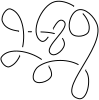
\includegraphics[width=.4\columnwidth]{tree_like.png}
    \caption{A tree-like curve.}
    \label{fig:treelike}
  \end{figure}
  Tree-like curves $\Rightarrow$ lower bound on unknottedness.
\end{frame}

\begin{frame}
  \frametitle{Tree-like curves}
    \begin{table}
    \centering
    \begin{tabular}{r|ccc}
      n & \# knot shadows & \# tree-like & \% tree-like \\
      \hline
      1 & 1               & 1            & 100.00\%     \\
      2 & 2               & 2            & 100.00\%     \\
      3 & 6               & 5            & 83.33\%      \\
      4 & 19              & 16           & 84.21\%      \\
      5 & 76              & 55           & 72.37\%      \\
      6 & 376             & 240          & 63.83\%      \\
      7 & 2,194           & 1149         & 52.37\%      \\
      8 & 14,614          & 6,229        & 42.62\%      \\
      9 & 106,421         & 35,995       & 33.82\%      \\
    \end{tabular}
    \caption{Counts of knot shadows and tree-like curves}
    \label{tab:counts}
  \end{table}
\end{frame}

\begin{frame}
  \frametitle{Unknottedness and tree-like shadows}
  \begin{figure}
    \centering
    \begin{tikzpicture}[scale=.75]
      \begin{axis}[
        ymode=log,
        log ticks with fixed point,
        title={Ratio of unknots, tree-like curves in $\le n$-crossing diagram iso. classes (log scale)},
        xlabel={Max \# crossings in diagram},
        ylabel={Percent},
        legend style={font=\tiny},
        legend pos=south west,
        legend entries={Unknots, Tree-like}
        ]
        \addplot table[x=n,y=unknot] {treelike.tsv};
        \addplot table[x=n,y=totrat] {treelike.tsv};
      \end{axis}
    \end{tikzpicture}

    \caption{The number of unknots is bounded by the number of
      tree-like diagrams.}
    \label{fig:unkdecay}
  \end{figure}
\end{frame}

\begin{frame}
  \frametitle{Delooped crossing number}
  \begin{table}
    \centering
    \begin{tabular}{r|c}
      $n$ & Average delooped crossing \# \\
      \hline
      3   & 0.50                         \\
      4   & 0.53                         \\
      5   & 0.92                         \\
      6   & 1.25                         \\
      7   & 1.72                         \\
      8   & 2.19                         \\
      9   & 2.70                         \\
    \end{tabular}
    \caption{Average delooped crossing number over shadows with $n$ crossings.}
    \label{tab:deloop}
  \end{table}
\end{frame}


% \begin{frame}
%   \frametitle{Prime knot shadows}
%   How many diagrams are connect sums? Prime?  [Figure]
% \end{frame}

\begin{frame}
  \frametitle{Questions to answer}
  \begin{block}{Conjecture}
    The ratio of unknots in diagrams tends to zero as $n$ increases.
  \end{block}
  This would match data from random curve experiments.
\end{frame}

\begin{frame}
  \frametitle{Questions to answer}
  Random curves project to diagrams.
  \begin{block}{Question}
    How does the pushforward measure differ from uniform diagram sampling?
  \end{block}
\end{frame}

\begin{frame}
  \frametitle{Questions to answer}
  \begin{block}{Question}
    Can we sample diagrams uniformly without enumeration?
  \end{block}
\end{frame}

\begin{frame}
  \frametitle{Future directions}
  \begin{itemize}
  \item Most analysis here is on knot diagrams; what can we say about
    link diagrams?
  \item How does the random diagram model compare to other models?
    \begin{itemize}
    \item \textit{Petaluma} model (Evan-Zohar, Hass, Linial, and
      Nowik)
    \item Random space polygons, random equilateral space polygons,
      random confined space polygons
    \item Random closed self-avoiding lattice walks
    \end{itemize}
  \item Uniform sampling of diagrams of higher crossing number: Can we
    avoid outright enumeration?
  \end{itemize}
\end{frame}

\begin{frame}
  \frametitle{Link diagrams}
  Counts for link diagrams
\end{frame}

\begin{frame}
  \frametitle{Knot distances}
  Can study pure knot theoretic things, not just probabilistic
  things--transitions between knots

  bat graph [figure]
\end{frame}

\section*{}

\begin{frame}
  \centering\textbf{\huge Thank you!}
\end{frame}


% \section{Definitions}
% \label{sec:def}
% \newcommand{\Salpha}[1]{S^2_{\alpha_{#1}}}

% \begin{frame}
%   \frametitle{Link shadows}
%   \begin{definition}
%     A \emph{link shadow} with $n$ vertices is an equivalence class
%     of connected 4-regular embedded planar multigraphs with $n$
%     vertices up to \emph{shadow isomorphism}.
%   \end{definition}

%   A shadow isomorphism is a graph isomorphism which preserves the
%   cyclic order of edges around each vertex.

% \end{frame}

% \begin{frame}
%   \frametitle{Examples of link shadows}

%   The following are four examples of link shadows.

%   \begin{center}
%     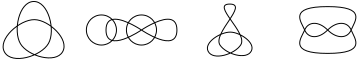
\includegraphics[width=4in]{linkshadow.pdf}
%   \end{center}

%   The leftmost and rightmost shadows are actually isomorphic shadows;
%   they differ in choice of exterior face.
% \end{frame}

% \begin{frame}
%   \frametitle{Components and knot shadows}
%   Two edges of a link shadow are said to belong to the same
%   \emph{component} if they meet at opposite ends of some vertex.

%   \begin{definition}
%     A link shadow is a \emph{knot shadow} if all edges in the shadow
%     belong to the same component.
%   \end{definition}

%   An \emph{orientation} on a component is a choice of directions on
%   edges in the component such that opposite edges meeting at a
%   vertex point head-to-tail.
% \end{frame}

% \begin{frame}
%   \frametitle{Link shadows and curves}
%   It is well understood that

%   \begin{proposition}
%     The (finite) set of knot shadows with $n$ vertices is in bijection
%     with the set of generic immersions of $S^1$ into $S^2$ up to
%     orientation-preserving diffeomorphisms of the sphere.
%   \end{proposition}
% \end{frame}

% \begin{frame}
%   \frametitle{Diagrams}
%   \begin{definition}
%     A \emph{link diagram} (or planar diagram) is a link shadow where
%     each component is oriented and each vertex is decorated with
%     over-under information for opposite edge pairs meeting at the
%     vertex, modulo \emph{diagram isomorphism}.
%   \end{definition}
%   \begin{itemize}
%   \item A diagram isomorphism is a shadow isomorphism which preserves
%     component orientation and vertex sign.

%   \item The decorated vertices are called \emph{crossings}.

%   \item If the underlying shadow of a link diagram is a knot shadow, then
%     we call it a \emph{knot diagram}.
%   \end{itemize}

% \end{frame}


% \section{The Database of Diagrams}

% \begin{frame}
%   \frametitle{Two (equivalent) tabulations}
%   \begin{itemize}
%   \item We first tabulate all link shadows, then expand the shadows
%     into diagrams.
%   \item Two independent methods to enumerate link shadows:
%     \begin{enumerate}
%     \item By taking duals of \emph{quadrangulations} of the sphere, or
%     \item By expanding planar simple graphs.
%     \end{enumerate}
%   \item Each method produces the same data.
%   \end{itemize}

% \end{frame}

% \begin{frame}
%   \frametitle{Dual quadrangulations}
%   Link shadows are 4-regular planar graphs, so their dual graphs are
%   quadrangulations.
%   \begin{definition}
%     A \emph{quadrangulation} is an embedded planar graph for which
%     every face has 4 (possibly not unique) edges. A quadrangulation is
%     \emph{simple} if it has no double edges.
%   \end{definition}
%   \begin{figure}
%     \begin{overpic}[width=4in]{quadrangulations-example.pdf}
%     \end{overpic}
%     \caption{\label{fig:QuadExamples} Examples of quadrangulations.}
%   \end{figure}
% \end{frame}

% \begin{frame}
%   \frametitle{Dual quadrangulations}
%   \begin{figure}
%     \hphantom{.}
%     \hfill
%     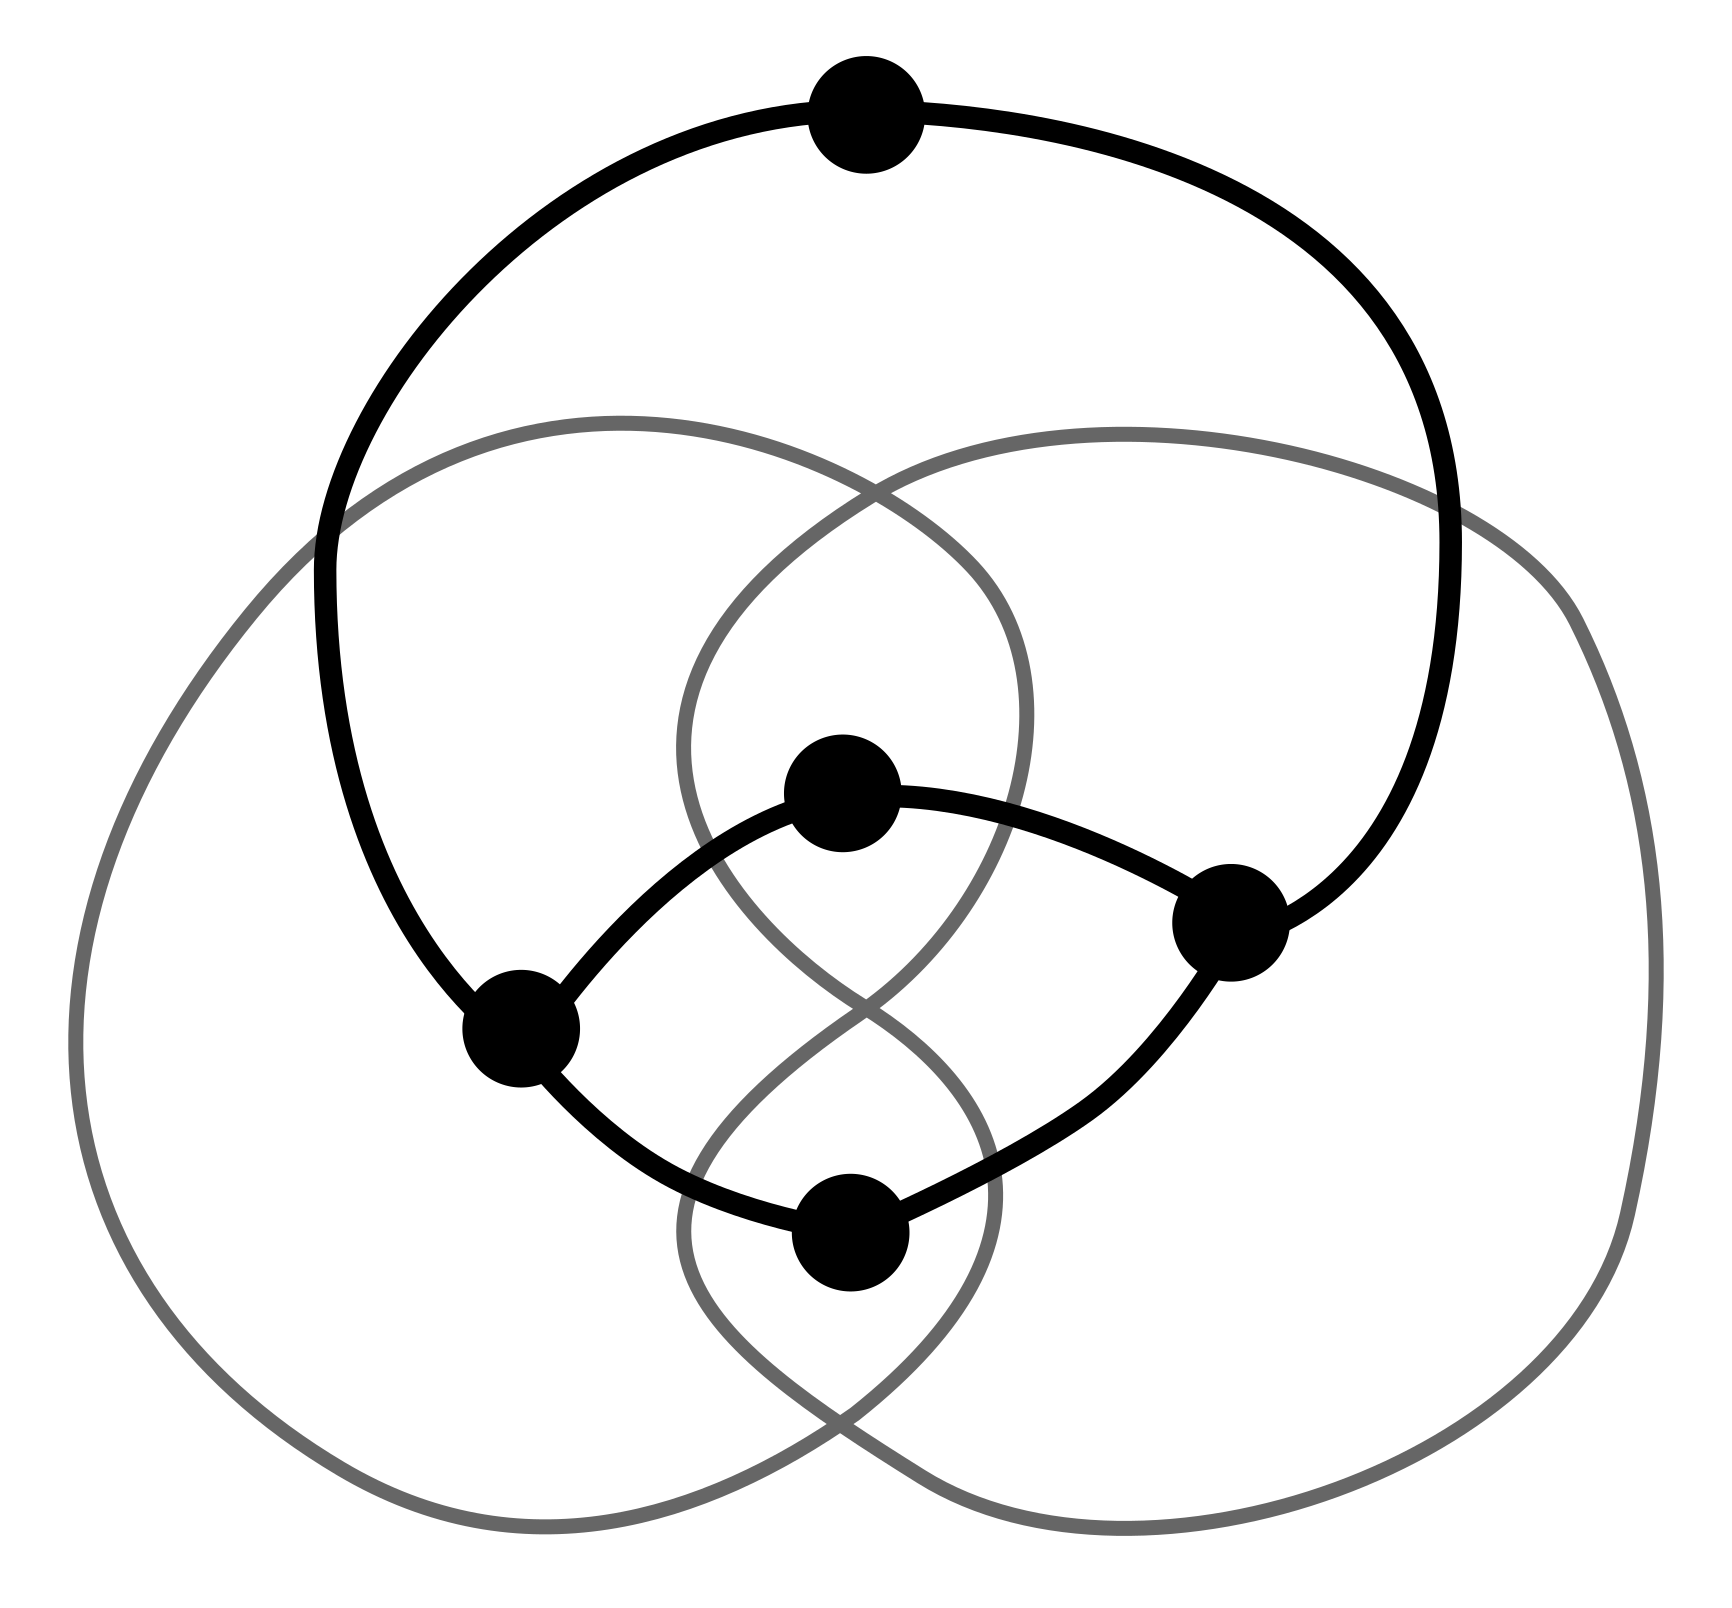
\includegraphics[height=1.25in]{quadrangulation} \hfill
%     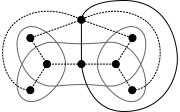
\includegraphics[height=1.25in]{non-simple-quadrangulation}
%     \hfill
%     \hphantom{.}
%     \caption{\label{fig:NonSimpleQuad} Two link shadows (gray) and their dual
%     quadrangulations (black)}
%   \end{figure}
% \end{frame}

% \begin{frame}
%   \frametitle{Prime diagrams}
%   \begin{definition}
%     Link shadows which have a simple dual quadrangulation are called
%     \emph{prime} diagrams. A shadow which is not prime is \textbf{composite}.
%   \end{definition}
%   Shadows which are composite can be realized as a \textit{shadow
%     connect sum} of two or more prime diagrams.
% \end{frame}

% \begin{frame}
%   \frametitle{Dual quadrangulations}
%   \begin{figure}
%     \hphantom{.}
%     \hfill
%     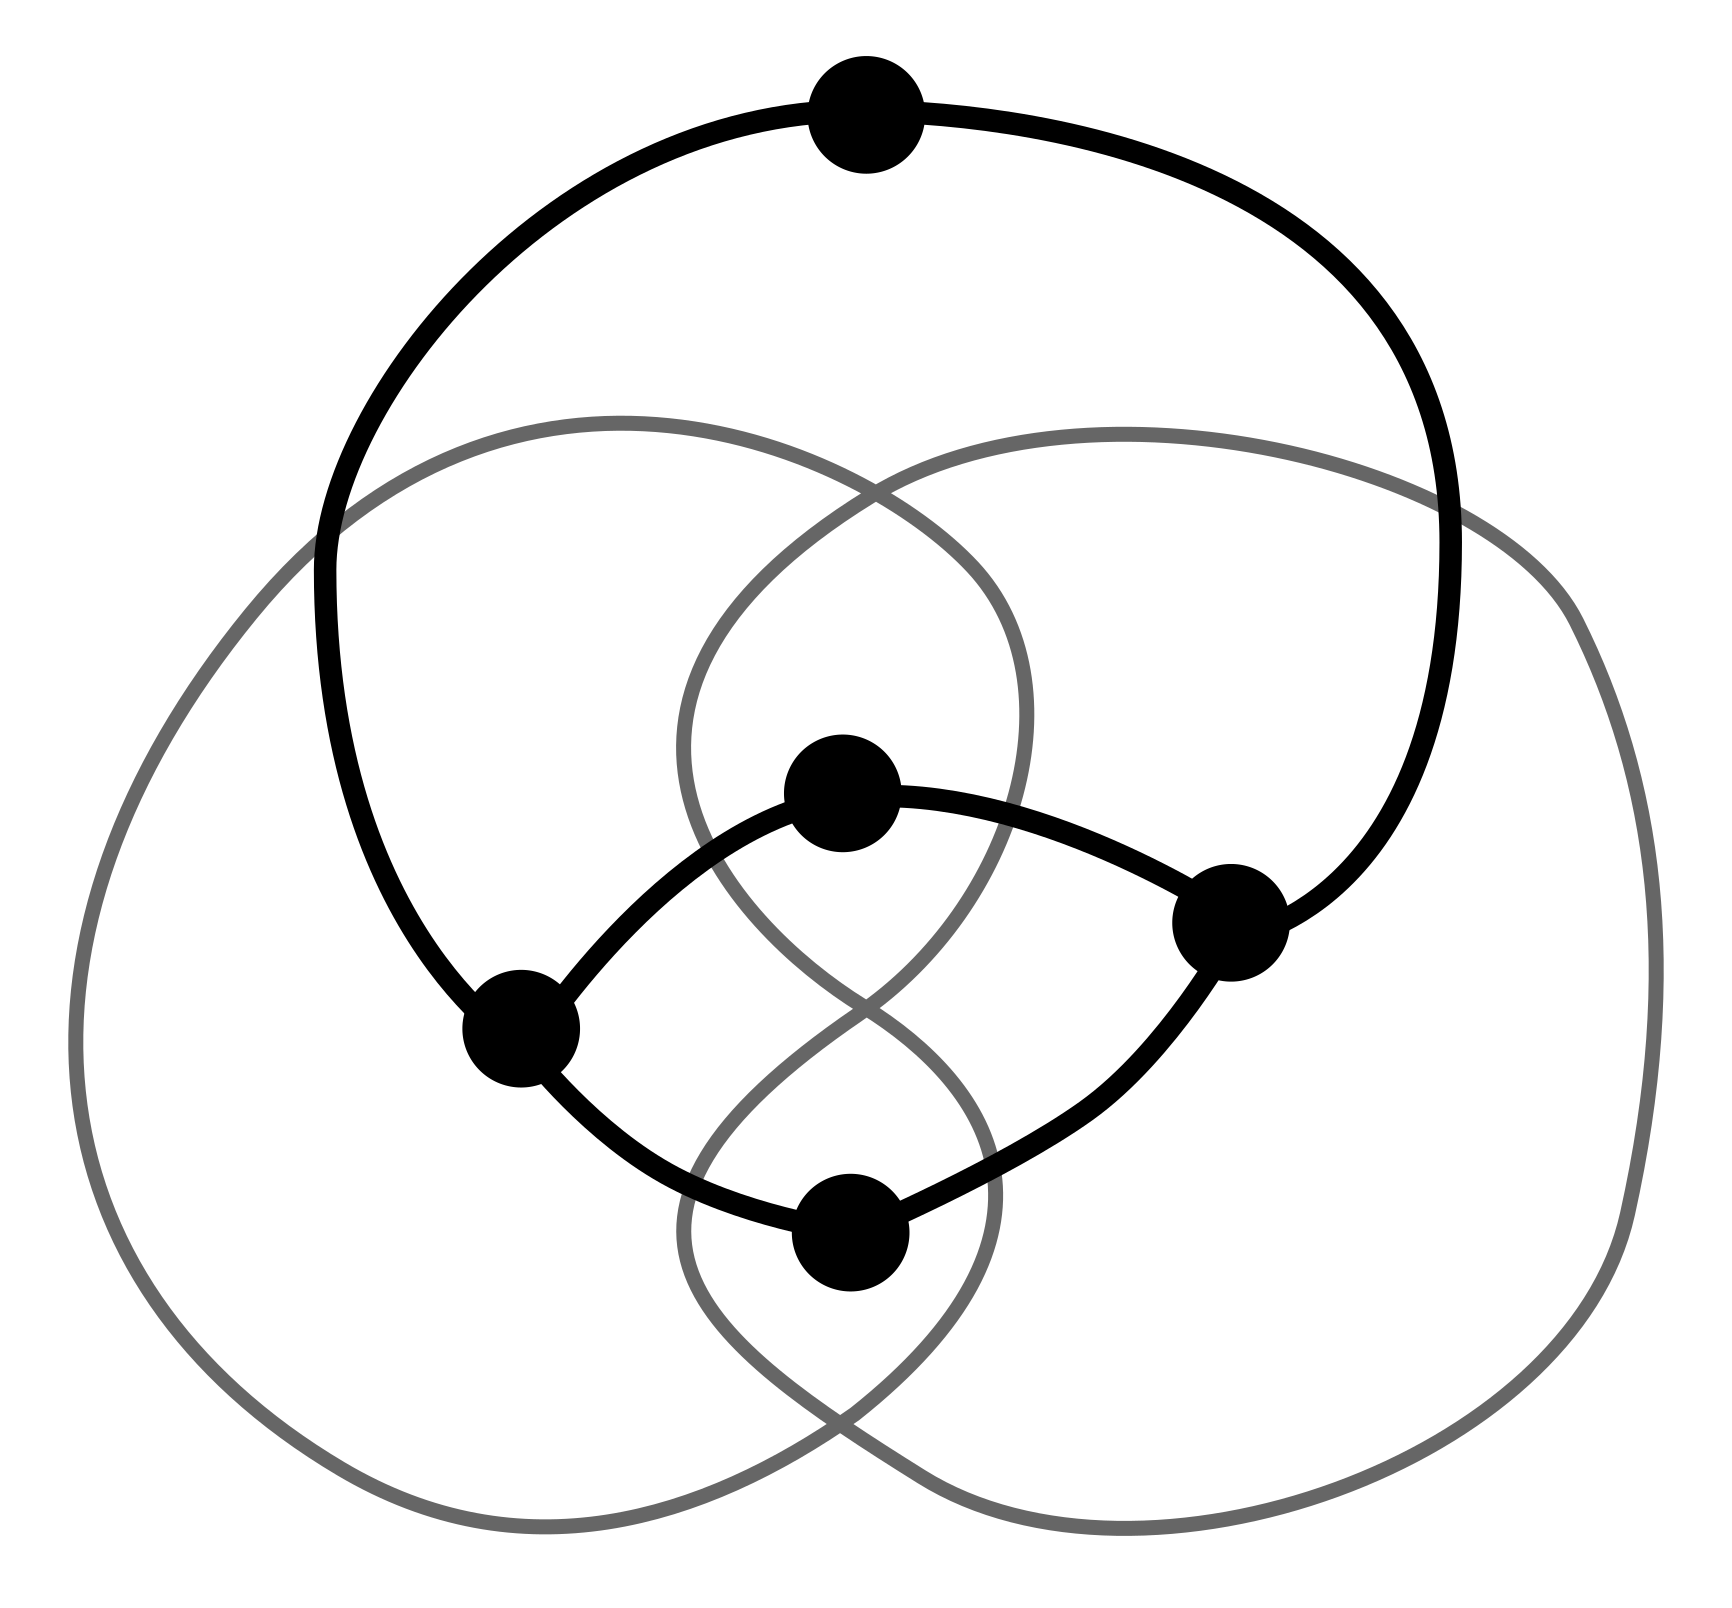
\includegraphics[height=1.25in]{quadrangulation} \hfill
%     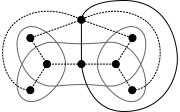
\includegraphics[height=1.25in]{non-simple-quadrangulation}
%     \hfill
%     \hphantom{.}
%     \caption{\label{fig:NonSimpleQuad2} Shadows and their duals. A
%       prime diagram (left), and a non-prime diagram (right).}
%   \end{figure}
% \end{frame}

% \begin{frame}
%   \frametitle{Enumerating all shadows}
%   \begin{enumerate}
%   \item The software \texttt{plantri} of Brinkmann and McKay is able
%     to generate all \textit{simple} quadrangulations (hence all
%     \textit{prime} diagrams).
%   \item Taking $k$-fold connect sums we can produce all diagrams, both
%     prime and composite.
%   \item Isomorphism checking to take only one representative per class.
%   \end{enumerate}
% \end{frame}

% \begin{frame}
% \frametitle{Quadrangulation enumeration workflow}
% \begin{center}
%   \begin{tikzpicture}[->,,shorten >=1pt,semithick,align=center,scale=.7]
%     %\tikzstyle{every node}=[align=center]
%     \node                  (prime2)
%     {Prime diagrams\\\tt{(plantri)}};
%     \node[left=.4in of prime2]  (prime1)
%     {Prime diagrams\\\tt{(plantri)}};
%     \node[right=.4in of prime2] (all)
%     {All diagrams\\of $n$ crossings};

%     \node[below=.5cm of prime2] (sum2) {2-summand\\diagrams};
%     \node[below=.5cm of sum2]   (sum3) {3-summand\\diagrams};
%     \node[below=1cm of sum3]    (sumn) {$n$-summand\\diagrams};

%     \path (prime1)    edge (prime2)
%                       edge (sum2.west)
%                       edge (sum3.west)
%                       edge (sumn.west)
%           (prime2)    edge (sum2)
%                       edge (all)
%           (sum2)      edge (sum3)
%           (sum2.east) edge (all)
%           (sum3)      edge[dashed] (sumn)
%           (sum3.east) edge (all)
%           (sumn.east) edge (all);
%   \end{tikzpicture}
% %\includegraphics[width=3in]{composite-workflow}
% \end{center}

% \end{frame}

% % \begin{frame}
% %   \frametitle{Graph expansions}
% %   \begin{itemize}
% %   \item The software \texttt{plantri} can also enumerate \textbf{simple}
% %     embedded planar graphs with $n$ vertices with given degree constraints.
% %   \item Link shadows are \textit{multigraphs}.
% %   \item Can amend the algorithm to enumerate all link shadows.
% %   \end{itemize}

% % \end{frame}

% % \begin{frame}
% %   \frametitle{Expansion procedure}
% %   \begin{enumerate}
% %   \item Set \texttt{plantri} to produce embedded planar simple
% %     connected graphs with maximum vertex degree 4.
% %   \item Expand planar simple graphs via a series of expansion moves
% %     $E_1, E_2, E_3, E_4$.
% %   \item Isomorphism checking to take only one representative per class.
% %   \end{enumerate}
% % \end{frame}

% % \begin{frame}
% %   \frametitle{Loop addition $E_1$}
% %     \begin{center}
% %     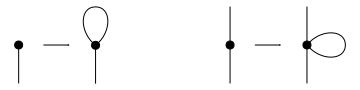
\includegraphics[width=4in]{loop-addition.pdf}
% %   \end{center}
% % \end{frame}

% % \begin{frame}
% %   \frametitle{Edge duplication $E_2$, $E_3$}
% %   \begin{center}
% %     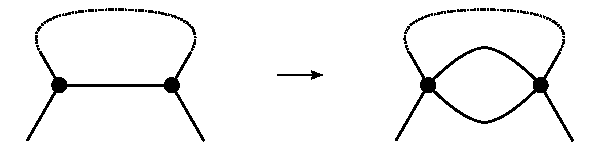
\includegraphics[width=4in]{edge-duplication-non-cut.pdf}
% %   \end{center}
% % \begin{center}
% %   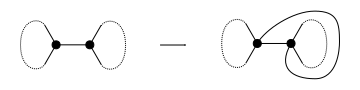
\includegraphics[width=4in]{edge-duplication-cut.pdf}
% % \end{center}
% % \end{frame}

% % \begin{frame}
% %   \frametitle{Pair insertion $E_4$}
% %   \begin{center}
% %     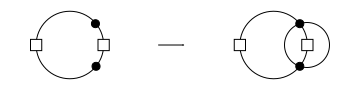
\includegraphics[width=4in]{pair-insertion.pdf}
% %   \end{center}
% % \end{frame}

% % \begin{frame}
% %   \frametitle{Expansion moves}
% %   \begin{proposition}
% %     Every link shadow $G$ can
% %     be obtained from a connected, embedded planar simple graph of
% %     vertex degree $\leq 4$ $G_0$ by a series of $\loopinsert$,
% %     $\edgedouble$, $\cutedgedouble$, and $\pairinsert$ expansions.
% %     \\\hfill \\
% %     Equivalently, link shadow $G$ can be reduced to a connected embedded planar
% %     simple graph $G_0$ of vertex degree $\leq 4$ by a series of
% %     $\loopinsert$, $\edgedouble$, $\cutedgedouble$, and $\pairinsert$
% %     reductions. The embedded isomorphism type of $G_0$ is determined
% %     by the embedded isomorphism type of $G$.
% %     \label{prop:reduce}
% %   \end{proposition}
% % \end{frame}

% % \begin{frame}
% %   \frametitle{Graph reduction}
% %   \begin{center}
% %     \includegraphics[width=4in]{expansion-from-simple-graph.pdf}
% %     % \caption{\label{fig:Expansion} An illustration of the process described in Proposition \ref{prop:reduce}}
% %   \end{center}
% % \end{frame}





\section{Additional information}
\bibliographystyle{alpha}


\end{document}

%%% Local Variables:
%%% mode: latex
%%% TeX-master: t
%%% End:
